\documentclass{standalone}
  \usepackage{tikz}
  \usetikzlibrary{arrows.meta, arrows}

  \begin{document}
    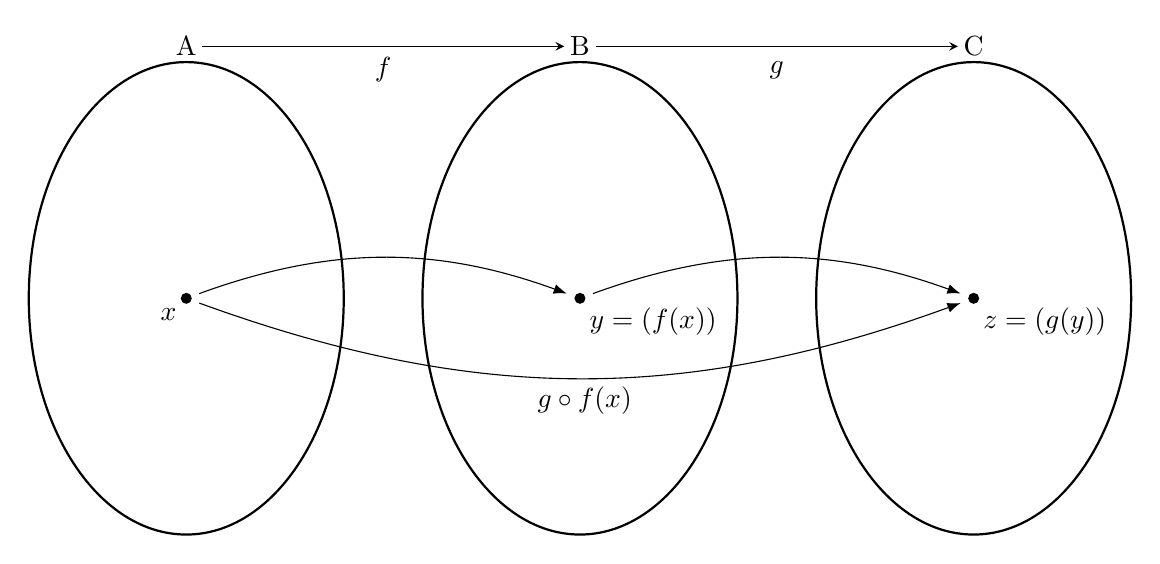
\begin{tikzpicture}

      \draw[thick] (0,0) ellipse[x radius=2, y radius=3]  +(0,3.2) node{A};
      \draw[thick] (5,0) ellipse[x radius=2, y radius=3] +(0,3.2) node{B};
      \draw[thick] (10,0) ellipse[x radius=2, y radius=3] +(0,3.2) node{C};

      \draw[-stealth] (0.2,3.2) -- (4.8,3.2) node[midway, yshift=-0.3cm]{$f$};
      \draw[-stealth] (5.2,3.2) -- (9.8,3.2) node[midway, yshift=-0.3cm]{$g$};
      
      \coordinate (x) at (0,0);
      \fill (x) circle[radius=0.07] node[below left] {$x$};

      \coordinate (y) at (5,0);
      \fill (y) circle[radius=0.07] node[below right] {$y=(f(x))$};

      \coordinate (z) at (10,0);
      \fill (z) circle[radius=0.07] node[below right] {$z=(g(y))$};


      \draw[-Latex, shorten <=5pt, shorten >=5pt] (x) to[in=160, out=20] (y);
      \draw[-Latex, shorten <=5pt, shorten >=5pt] (y) to[in=160, out=20] (z);
      \draw[-Latex, shorten <=5pt, shorten >=5pt] (x) to[in=-160, out=-20] (z) node[below left, xshift=-120, yshift=-1cm] {$g \circ f(x)$};

    \end{tikzpicture}
  \end{document}